\section{Introduction}
\label{secall:intro}
The first ideas about heavy-ion experiments at the Large Hadron Collider (LHC)~\cite{Evans:2008zzb} at CERN were formed in the late eighties and the early nineties~\cite{Jarlskog:1990dv}. Since the beginning of the LHC project, approved by CERN Council in 1994, the investigation of heavy-ion collisions has been an integral part of the LHC physics programme. Built from 1998 to 2008 in the 27~km long circular underground tunnel, earlier exploited by the Large Electron--Positron (LEP) collider, the LHC machine represents the highest-energy particle accelerator ever made. This very versatile collider is designed to reach centre-of-mass energies up to $\sqrt{s} = 14$~TeV for proton--proton (pp) collisions, and up to 1\,150~TeV using lead-ion beams, corresponding to $\sqrt{s_{\rm NN}} = 5.5$~TeV per colliding nucleon pair. These will entail the energy increase by a factor of seven for hadron collisions, and and more than 27 for heavy-ion collisions compared to previous colliders.
\subsection{Physics motivation}
\label{subsecall:motivation}
At very high temperatures and densities, hadronic matter is expected to undergo a phase transition into a qualitatively different state, where quark and gluon degrees of freedom are liberated. Such conditions were prevailing in the early Universe, a few microseconds after its formation. In heavy-ion collisions at ultra-relativistic energies, nuclear matter is heated and compressed reaching conditions well beyond the phase-transition point, and the same type of medium filling the very early Universe is thus momentarily re-created. At the highest available energies, at the LHC, far better conditions, than those at the other existing facilities, are achieved to study this state of matter, called the Quark--Gluon Plasma (QGP). The nearly-vanishing baryon density, the highest available initial temperature and energy density, and the abundance of perturbatively-calculable hard Quantum Chromo-Dynamics (QCD) processes make heavy-ion collisions at the LHC particularly well-suited for precision studies of the QGP properties.

QCD, the well-established theory of strong interactions, predicts (cross-over) phase transitions in strongly interacting matter at high temperatures. A phase transition reflects breaking of a fundamental symmetry in the theory. Above the critical temperature, ordinary hadronic matter, where protons and neutrons are composed of quarks and gluons confined in a colour-neutral state, melts during the deconfinement phase transition. In the deconfined medium, quarks and gluons are not bound into hadrons anymore, however, the effective degrees of freedom of the QGP, formed at temperatures achieved with heavy-ion collisions, are rather complex. A second phase transition is connected with the generation of hadron masses as a consequence of the presence of a quark--antiquark condensate in the vacuum at low temperature. According to QCD, at high temperatures, the vacuum condensate is reduced, and the masses of quarks drop to their bare values during a chiral phase transition. Quantitative lattice QCD calculations~\cite{Borsanyi:2010bp} confirm that QCD matter undergoes a transition from a hadronic gas to a QGP at a temperature about 160~MeV, corresponding to an energy density of about 0.5~GeV/fm$^3$. At LHC conditions (low baryon density), the transition is a smooth cross-over spanning a temperature range of 20--30~MeV, which means that the precise value of the critical temperature depends on the observable used to locate it.

In a heavy-ion collision the energy deposited at mid-rapidity is determined by the density of low-$x$ (Bjorken $x$, corresponds approximately to the fraction of nucleon longitudinal momentum carried by a parton) gluons confined in the colliding nuclei. The relevant values of $x$ at LHC energies are one order of magnitude smaller than those at RHIC, i.e. on the $10^{-3}$ level and below. In such small-$x$ range, at low virtualities the perturbative gluon distribution reaches saturation and gluons have to fuse, in order not to violate unitarity.  This marks the transition to the non-linear parton-evolution region, and the virtuality scale at which this transition happens is known as the saturation scale $Q_{\rm s}$. It increases (logarithmically) with the incident energy, and the mass of colliding nuclei (as the nucleon radius), and  reaches values $Q_{\rm s} \approx 3$--$4$~GeV$^2$ for Pb--Pb collisions at the LHC. During the collision of the two nuclei, these dense gluon fields are deconfined and create a primordial strongly-interacting medium, which rapidly expands and thermalizes. The thermalized QGP continues to cool down, mainly by longitudinal expansion, until its temperature decreases below the critical temperature of the QCD phase transitions, and then it is converted into a gas of hadron resonances. At this moment the produced-particle composition is frozen. The corresponding temperature is called the chemical freeze-out temperature ($T_{\rm ch}$), and is presumably rathe close to the critical temperature of the QCD phase transitions. Hadrons after chemical freeze-out continue to interact. However, since their relative energy is below the threshold for inelastic production, only their momentum spectra are modified. At kinetic freeze-out, with corresponding kinetic freeze-out temperature ($T_{\rm kin}$), the medium is so diluted that the final hadrons cease interacting altogether and decouple.

Prior to the start-up of the LHC heavy-ion programme, the nature of the QGP as an almost-perfect, inviscid liquid emerged from the experimental investigations at RHIC~\cite{Tribble:2007nsac}. The pressure created in the thermalized QGP phase is reflected in the large azimuthal asymmetry observed in the final-state particle production. The resistance of the medium  to the shape change implies a very low shear viscosity, or in dimensionless variable, a very low ratio of shear-viscosity to entropy-density in the QGP. This indicates extremely short mean-free path inside the medium at this stage of the evolution (and the corresponding cross section approaching the unitarity limit) induced by complex excitation modes in the strongly-coupled QCD medium. This also implies the development of a collective transverse velocity field already at this stage contributing to the plasma cooling. The smallness of the mean-free path with respect to the system size allows for the successful utilization of relativistic hydrodynamics in the description of the evolution of the thermalized QGP until hadronization.

Such an interpretation is further supported by the observation of the strong energy loss of partons traversing this strongly-coupled QCD medium, demonstrated at RHIC with large suppression of particle production at transverse momenta ($p_{\rm T}$) up to 20~GeV. Deduced from these measurements, the large amount of the energy lost by hard partons due to gluon bremsstrahlung and by elastic collisions is consistent with the low shear viscosity established from the collective-flow pattern of low-momentum hadrons. With the first LHC data, this basic picture has been confirmed with the observation of deconfined matter at unprecedented values of temperatures, densities and volumes~\cite{Muller:2012zq}. The origin and properties of this almost-perfect-fluid QGP behaviour  is the subject of further experimental study at the LHC. Among the important questions to answer are: does the predicted initial gluon saturation also reduce the low-$p_{\rm T}$ particle yields?; is the low shear viscosity affected by the expected increase of the QGP temperature at an early stage? However, the most important impact of the more than one order of magnitude increase of the collision energy is the large increase of the rates for hard probes, such as the jets, electro-weak particles, heavy flavours, and quarkonia. The high rates allow for precision studies of the QGP using the in-medium interactions of these probes, better controlled theoretically than the propagation of light partons. In addition, some observables, e.g. very high-energy jets, electro-weak bosons, and different $\Upsilon$ states, are accessible in heavy-ion collisions for the first time. A comprehensive compilation of theoretical predictions for the LHC heavy-ion programme was published in~\cite{Abreu:2007kv}.

The experimental results obtained using heavy-ion collisions during the first period of the LHC running are summarized in this article. It is divided into sections according to the various observables: Sec.~\ref{secks:eventchar} describes the principles of centrality selection and measurements of particle and energy densities; particle yields and spectra are discussed in Sec.~\ref{secks:spectra}; correlation studies are illustrated in Sec.~\ref{secks:nonflow} for non-flow effects, and in Sec.~\ref{sec:ps:flow} for flow phenomena; Sec.~\ref{sect:pas:ew} deals with the production of electro-weak bosons; Sec.~\ref{jets_intro} is dedicated to jets and their quenching; two sections are devoted to heavy flavours, Sec.~\ref{secks:heavy} to open heavy flavours, and Sec.~\ref{sec:qurkonia} to quarkonia. Summary and outlook are given in Sec.~\ref{secall:summary}.

\subsection{LHC heavy-ion running}
\label{subsecall:running}

\begin{figure}[!htb]
\begin{center}
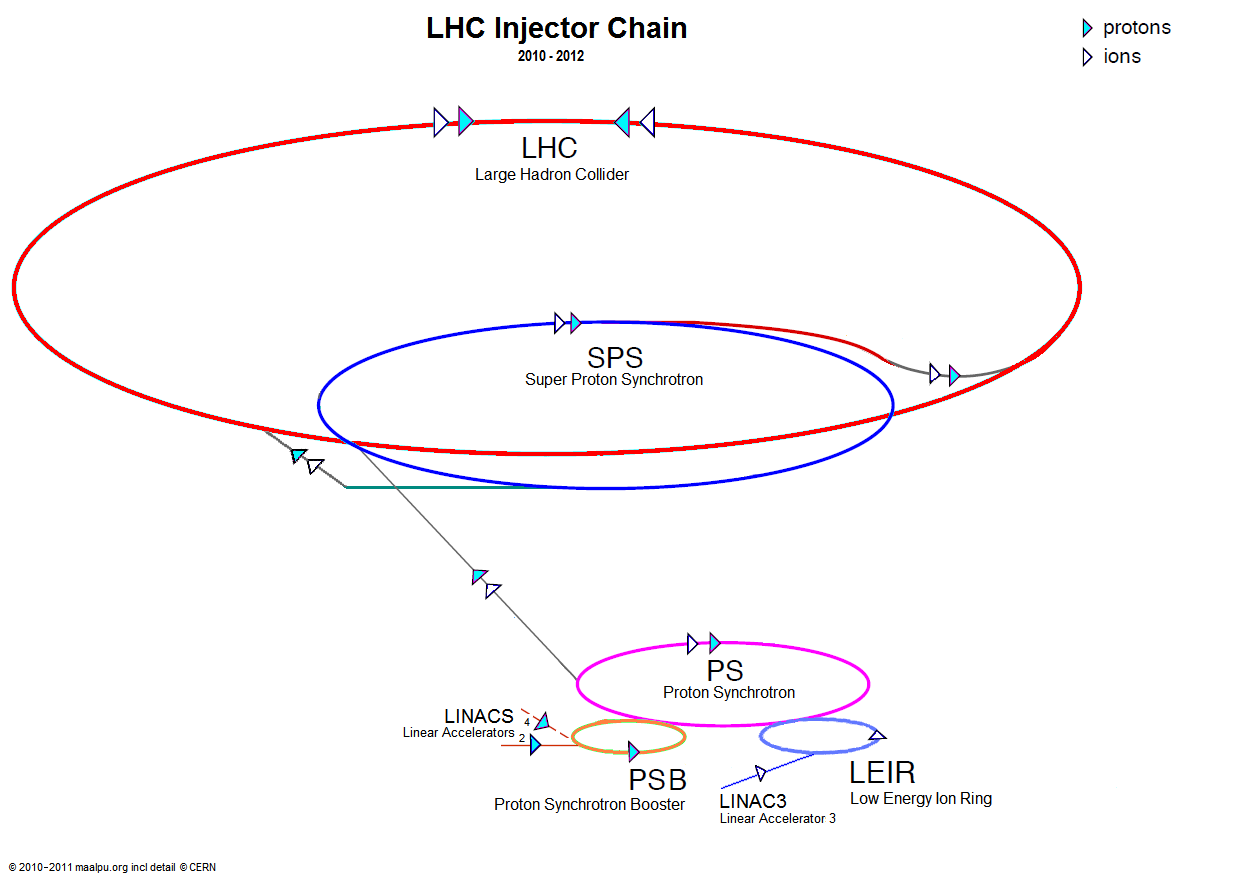
\includegraphics[width=0.8\textwidth]{introduction_figs/LHC_chain.png}
\caption[]{Schematic view of LHC injector chain, showing the path of both protons and ions.}
\label{fig:pas:intro:lhc}
\end{center}
\end{figure}

Heavy ion running at the Large Hadron Collider had been planned long before the machine was built.
This was based on the interest in the physics at the CERN SPS, which was colliding light ions since
1986 and heavy ions since 1994, and as a natural extension to the already-planned program
at the Relativistic Heavy Ion Collider (RHIC).
The accelerator complex is shown in Figure~\ref{fig:pas:intro:lhc}.
Ions start their path to collisions at the ECR (electron cyclotron resonance) ion source,
which provides lead isotope $^{208}$Pb ions stripped to values around Pb$^{29+}$, which are passed through
a spectrometer to select Pb$^{29+}$ and accelerated in a linear accelerator to 4.2 MeV/n.
They are then stripped to around Pb$^{54+}$ by a 0.3 $\mu$m carbon foil and the
Pb$^{54+}$ are selected by a spectrometer to be fed into the CERN Low Energy Ion Ring (LEIR).
LEIR is used to transform a set of low intensity ion pulses from the LINAC into shorter
bunches with higher intensity.  This is done by filling the available phase space in
three dimensions.  After this, electron cooling is applied to shrink the beam to increase the
bunch density, and decelerate it into ``a stack sitting slightly inside the central orbit''.
At this point, seven pulses are captured, split into two bunches, and then accelerated to
72 MeV/n.
The bunches from LEIR are then sent to the CERN PS (Proton Synchrotron), accelerated to
5.9 GeV/n and stripped fully to Pb$^{82+}$ using a 0.8 mm aluminium foil.  These ions
are then sent to the SPS where they are accelerated to 177 GeV/n and injected into the LHC.

To date, there have been three heavy ion runs at the LHC.
The first run was in November--December 2010,
which provided 120 colliding bunches of lead ions in each ring, with a center of mass energy per nucleon
pair of $\energy =2.76$~TeV, a peak luminosity of $3 \times 10^{25} \mathrm{cm}^{-2} \mathrm{s}^{-1}$ and an integrated luminosity
of 7~$\mu \mathrm{b}^{-1}$, corresponding to about 50 million minimum bias events.
The second run was in November--December 2011, which provided about 360 colliding bunches of lead ions per ring,
also at $\energy =2.76$~TeV, a peak luminosity of
about $5 \times 10^{26} \mathrm{cm}^{-2} \mathrm{s}^{-1}$ and an integrated luminosity of
about 150~$\mu \mathrm{b}^{-1}$, a factor of 20 increase over 2010.
The third run, in January--February 2013, provided proton-lead collisions
at $\energy=5.02$~TeV but these results are not discussed
in detail in this review.

\subsection{Detectors at the LHC}
\label{subsecall:detectors}

Three, out of the four principal LHC detectors, participate in the LHC heavy-ion programme. These are: ALICE (A Large Ion Collider Experiment), a dedicated heavy-ion detector designed to operate in the high particle density environment; and two general-purpose particle detectors, ATLAS (A Toroidal LHC ApparatuS) and the CMS (Compact Muon Spectrometer), optimized to high interaction rates and capable of precision measurements at very high transverse momenta. The fourth detector, the LHCb, was not taking data in Pb--Pb runs due to the occupancy limitation, however, it participated in the p--Pb run, and reported interesting results.

\subsubsection{ALICE}

\begin{figure}
\begin{center}
\includegraphics[height=0.49\textwidth]{introduction_figs/ALICEdet.png}
\caption{Schematic layout of the ALICE detector, indicating the main subsystems. The inset in the top-right corner shows the innermost part in detail.}
\label{figks:ALICEdet}
\end{center}
\end{figure}


The ALICE detector~\cite{Aamodt:2008zz} is shown in Fig.~\ref{figks:ALICEdet}, it has the following main parts: central barrel, muon arm, and forward detectors. The central barrel is housed in a large solenoid magnet providing the field of 0.5~T, with 12~m aperture and 12~m length, which was inherited from the L3 experiment running at the LEP collider. This part provides measurements of particles produced within about $\pm 45^\circ$ with respect to a plane perpendicular to the beam axis, corresponding to the pseudorapidity coverage $|\eta| < 0.9$ ($\eta = - \ln \tan (\Theta/2)$, where $\Theta$ is the angle from the beam axis). The six-layer silicon Inner Tracking System (ITS), surrounding the beryllium vacuum beam pipe of 6~cm diameter, begins with pixel detectors at radii 4 and 8~cm, continues with silicon-drift detectors at 14 and 22~cm, and ends with double-sided strip detectors at 39 and 43~cm. The ITS measures the particle tracks with position precision of a few tens of microns. In addition, the four outer layers participate in the Particle Identification (PID) by determining the specific ionization energy loss (${\rm d}E/{\rm d}x$). The excellent spatial resolution of the innermost silicon pixel layers results in outstanding capabilities of primary and secondary vertex reconstruction.  The resolution in measuring the distance of closest approach to the primary vertex for tracks coming from secondary decays with transverse momentum \pT\ of 1~GeV is in the range 60--70~$\mu$m, allowing to detect weak decays of charm and beauty particles.
The main particle tracking device is the TPC (Time Projection Chamber), the largest such detector built to date. It has a cylindrical shape and a size of more than 5~m along the beam axis, and 5~m in outer diameter. The TPC continues the tracking from the ITS starting from a radius of 88~cm and carries on till its outer radius of 2.5~m. The TPC volume, filled with neon-based gas mixture, is divided into two halves by a thin central high-voltage electrode providing an electrostatic field of about 0.4~kV/cm. Electrons created by ionization in the gas drift towards one of the end-plates equipped with multi-wire proportional chambers with cathode-pad readout. Altogether the TPC is read out with more than 600~thousands pads, which gives, taking into account the sampling along the drift direction, an effective granularity in the TPC volume of more than half a billion three-dimensional pixels. This results in very efficient track-finding down to low transverse momenta, about 100~MeV, even at the highest particle densities in central lead--lead collisions at LHC energies. In addition, the ALICE TPC has an excellent resolution for the measurement of ${\rm d}E/{\rm d}x$; between 5 and 6\,\%, depending on particle density.
The momentum dependencies of ${\rm d}E/{\rm d}x$ for different particles come close together when approaching their minima for ionization energy losses. This makes particle identification using the above method impossible in that momentum region. To distinguish particle species in this region, ALICE installed a Time-Of-Flight detector (TOF) at a radius of about 3.7~m from the beam axis. This detector determines the arrival time of charged particles with a precision better than 100~ps, exploiting multi-gap resistive plate chambers, an innovative technology developed specifically for ALICE. The TOF measurement is able to separate pions and kaons up to 2.2~GeV, K mesons and protons up to 3.5~GeV, and can be used for electron identification at lower momenta. To further increase the momentum reach for charged hadron identification, a smaller detector, the High-Momentum PID (HMPID), covering about 10\,\% of the area covered by the other central barrel detectors and using the \v{C}erenkov ring-imaging technique, is placed at a distance of 1~m larger than that of TOF. To improve the electron identification ALICE uses a Transition Radiation Detector (TRD) situated between the TPC and TOF detectors. Particles traverse six radial drift chambers, each consisting of a transition radiator followed be a volume containing a xenon-based gas mixture, allowing the detection of X-ray photons in addition to charged tracks. The TRD drift chambers are read out with cathode-pad wire chambers. Electrons are separated from pions by discriminating on the signal amplitude of last samples, where the electron transition radiation contributes. This detector is also used in the tracking; an increase of the track length in the magnetic field improves the momentum resolution at high transverse momenta (to about 5\,\% around 100~GeV). At low momenta, 0.1--1~GeV, the momentum resolution of the ALICE tracking system is better than 1\,\%. The central barrel part of ALICE is completed with electromagnetic calorimeters. The larger one, EMCal, covers $120^\circ$ in azimuthal angle, and in the longitudinal direction, a little less than the barrel detectors in front of it. It is used to trigger on jets and to improve the jet energy determination measured with tracking detectors. The much smaller Photon Spectrometer (PHOS) has significantly better energy resolution and granularity, and is dedicated to the isolation of a direct photon signal in heavy-ion collisions.

The ALICE detector can detect and trigger on muons in the forward region on one side of the central barrel using its muon arm, between $2^\circ$ and $9^\circ$ from the beam axis. A conical absorber begins at only 90~cm from the nominal interaction point, in order to suppress the background from decaying pions and kaons. Behind the absorber, five tracking stations detect the filtered-out muons. The first two stations are located inside the main solenoid magnet; the third one is in the middle of a dipole magnet with 3~Tm of field integral used for muon momentum analysis; the remaining two measure deflected muon tracks behind the dipole. Each tracking station consists of two planes of multi-wire chambers with cathode-pad readout, giving a coordinate precision of about 100~$\mu$m in the bending plane, thus giving a mass resolution of 1\,\% at the $\Upsilon$ mass, needed for the separation of the different $\Upsilon$ states. Behind the last muon tracking station a second absorber shields the muon trigger detectors from the surviving  background. Two trigger planes of Resistive Plane Chambers (RPC) detect the position and direction of penetrating muons. Using this information the muon trigger electronics select events having muons with transverse momentum above a predetermined threshold. The full length of the muon arm, from the interaction point to the end of the trigger system, is about 20~m.

On the side opposite to the muon arm the Photon Multiplicity Detector (PMD) measures the yield of $\pi^0$ mesons by counting the number of photons. The Forward Multiplicity Detector (FMD), with silicon strip planes on both sides of the interaction region, determines the density of charged particles emitted at pseudorapidities $-3.4 < \eta -1.7$ and $1.7 < \eta < 5$. Scintallator tile arrays (VZERO), covering an acceptance similar to to that of the FMD, are used to trigger on LHC collisions, selecting different centrality classes with corresponding thresholds. Small quartz counters on both sides (TZERO detector) are employed in time-of-flight measurements. Zero Degree Calorimeters (ZDC) are placed more than 100~m from the interaction region in both directions; on each side there is one for the detection of proton spectators and one for neutron spectators.



\subsubsection{ATLAS}

\begin{figure}[!htb]
\begin{center}
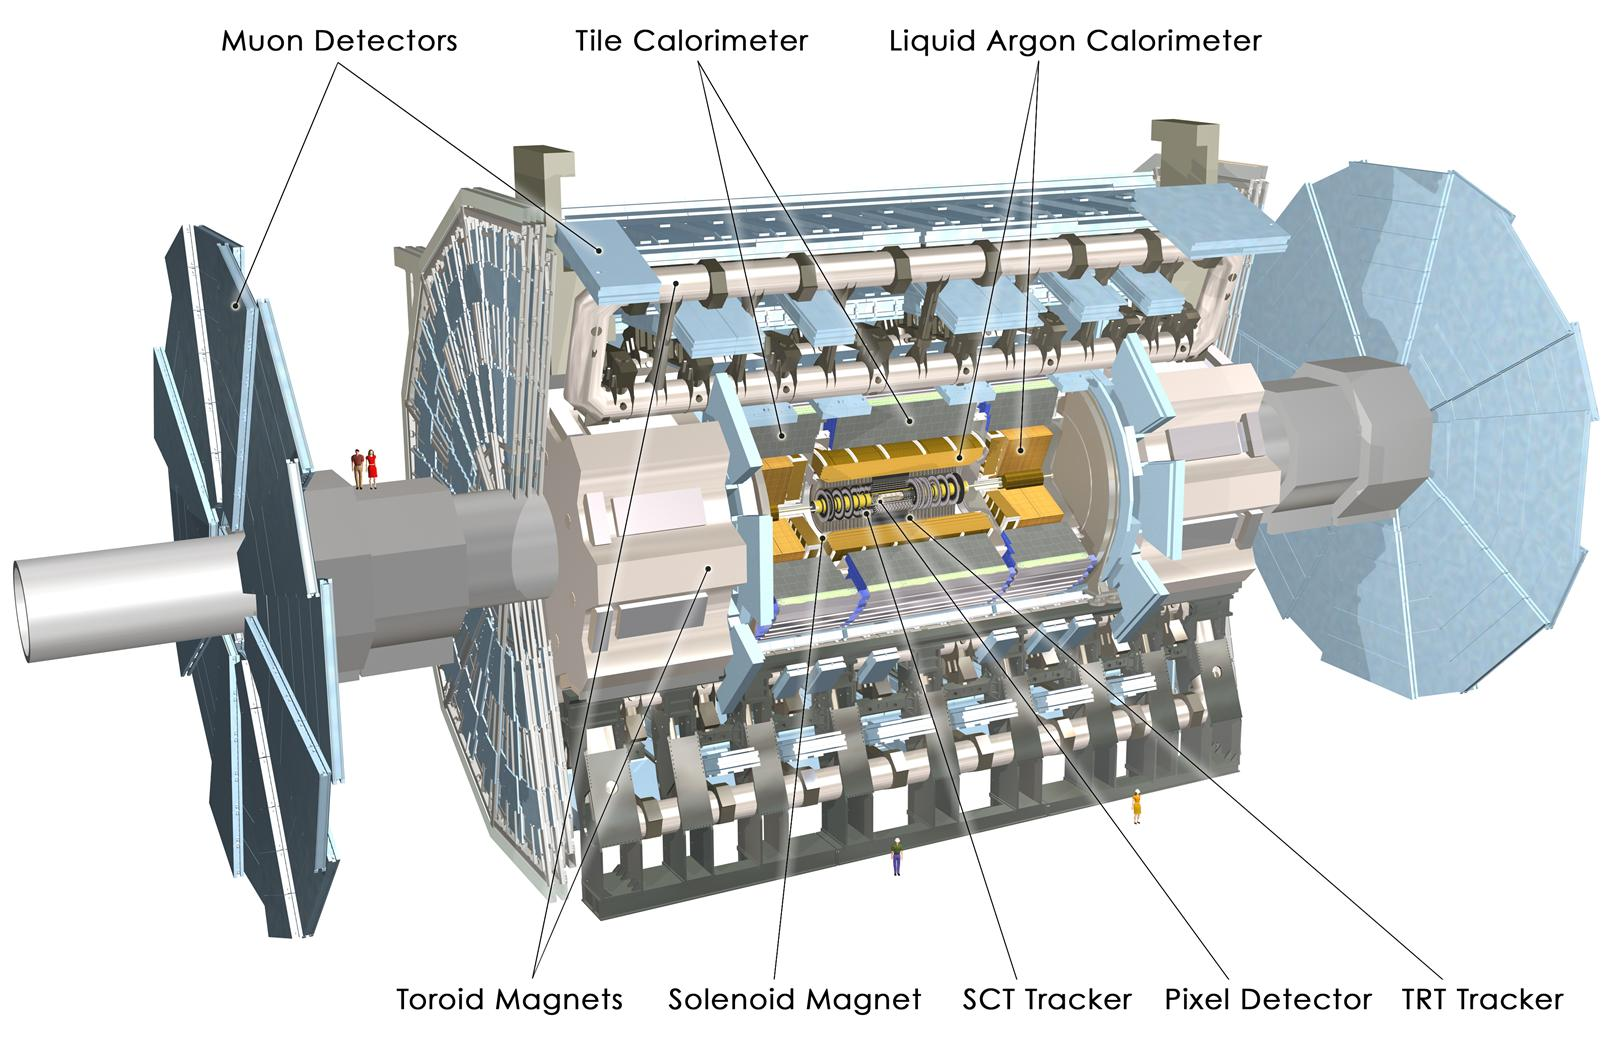
\includegraphics[height=0.49\textwidth]{introduction_figs/0803012_05-A4-at-144-dpi.jpg}
\caption[]{Schematic view of ATLAS detector at the LHC, highlighting the major subsystems.}
\label{fig:pas:intro:atlas}
\end{center}
\end{figure}

%ATLAS
The ATLAS detector~\cite{Aad:2008zzm}, shown in Figure~\ref{fig:pas:intro:atlas} is one of the general-purpose particle physics
detectors at the LHC.
It has three main detector systems: the inner detector (ID), the calorimeter,
and the muon spectrometer (MS).
%
The inner detector tracks charged particles using three separate detector
technologies, and the spectrometer is immersed in a 2~T axial field from a
superconducting solenoid magnet 1.2~m from the nominal beam axis.
The pixel detector typically provides three high-resolution space points
with three layers of pixel detector surrounding the beam pipe within
$|z|<400$~mm (covering approximately $|\eta|<2$ and 4 disks at forward
angles covering out to $|\eta|<2.5$.
The detector has approximately 80.4 million readout channels.
While the minimum pixel size is $50 \times 400$~$\mu$m$^2$, the intrinsic
position resolution is 10~$\mu\mathrm{m}$ in $R-\phi$ and 115~$\mu\mathrm{m}$ in $z$
in the barrel region, and 10~$\mu\mathrm{m}$ in $R-\phi$ and 115~$\mu\mathrm{m}$ in $R$
in the disks.
The semiconductor tracker detector (SCT) consists of silicon strips covering out to
$|\eta|<X$ in the barrel region and $|\eta|<2.5$ in the forward regions.
The detector has approximately 6.3 readout channels.
The sensors have 80~$\mu$m pitch and are
double-sided with a 40~mrad angle between the strip
directions to measure hit positions in two dimensions.
The intrinsic accuracies per module are
17 $\mu\mathrm{m}$ in $R-\phi$ and 580  $\mu\mathrm{m}$ in $z$
in the barrel region, and 17 $\mu\mathrm{m}$ in $R-\phi$ and 580  $\mu\mathrm{m}$ in $R$
in the disks.
The transition-radiation tracker (TRT) covers $|\eta|<2$ with 351,000 4 mm straw tubes in
both the barrel and forward regions.
It only provides $R-\phi$ coverage out to $|\eta|=2.0$, with tubes parallel to the beam
axis in the barrel region and arranged radially in the endcaps.
A track typically has three hits in the pixel detector, 7 hits in the SCT, and 36 in the
TRT.

%
The ATLAS calorimeter has large coverage in pseudorapidity ($|\eta|<4.9$)
and longitudinal segmentation in both electromagnetic and hadronic
sections.
In the barrel region, the electromagnetic calorimeter uses lead as an absorber
and liquid argon (LAr) as the sampling material.
The kapton electrodes and lead absorber are accordion shaped over the full
coverage, providing full coverage in $\phi$ without cracks.
The EM calorimeter has three longitudinal sections and a presampler layer.
The first layer has very high resolution
in the $\eta$ direction, allowing discrimination of photons from
neutral hadron decays.
The second layer is coarser but deeper, providing the primary energy
measurement for electromagnetically interacting particles (photons and
electrons), while the third layer is there to catch the tails of the
deposited electromagnetic showers.
It has a barrel section covering $|\eta|<1.475$ and two endcap sections
each housed in their own cryostat.  The outer endcap covers $1.375<|\eta|<2.5$
and the inner wheel covers $2.5<|\eta|<3.2$.
%
The ATLAS hadronic calorimeter uses steel absorber and measures the
hadronic shower energy using scintillating tiles.
It has a barrel region covering $|\eta|<1.0$ and an extended barrel
covering $0.8 < |\eta|< 1.7$.
Radially, the calorimeter extends from 2.28 m to 4.25 m.  It
has three longitudinal sections, which are 1.5, 4.1 and 1.8 interaction
lengths thick for the barrel region and 1.5, 2.6 and 3.3 interaction
lengths thick for the extended barrel.
%
The hadronic end-cap covers $1.5 < |\eta|< 3.2$ and uses LAr technology
similar to the EM calorimeter but with copper absorber.
%
The ATLAS forward calorimeter (FCal) covers $|\eta|=3.2-4.9$, using
a matrix of copper and liquid argon in the electromagnetic section,
and tungsten and liquid argon for the hadronic section.
The FCal has a depth of about 10 interaction lengths.
%

The ATLAS muon spectrometer covers $|\eta|<2.7$ and is divided into
barrel and endcap regions, which are covered by different configurations
of magnets and detector technologies.
The bending of muons is provided by three sets of air-core toroids,
a barrel toroid covering $|\eta|<1.4$ and providing 1.5-5.5 Tm of bending power,
and two end-caps regions covering $1.6 < |\eta| < 2.7$ with 1-7.5 Tm of
bending power.  The region $1.4 < |\eta| <1.6$ is covered by
a combination of both sets of magnetic fields.
The barrel region has tracking detectors arranged in three cylindrical
layers around the beam axis, while in the forward region, chambers are
arranged in three layers perpendicular to the beam.
Out to $|\eta|=2$, track positions are measured using Monitored Drift Tubes (MDTs).
Beyond $|\eta|=2$, multiwire Cathode Strip Chambers (CGC) with higher granularity
are used.
The muon system provides a momentum resolution ranging from approximately 2\% at
low \pT up to about 10\% at $\pT=1$ TeV.
%

Two sets of forward detectors are used for minimum-bias triggering in both
p+p and Pb+Pb running.  The Minimum Bias Trigger Scintillators (MBTS) are
2 cm thick polystyrene slats mounted at $z=3.6$ m, divided into 8 sections in
$\phi$ and two sections in $\eta$, covering $2.09<|\eta|<2.82$ and
$2.82<|\eta|<3.84$.  They are read out by wavelength-shifting fibers embedded
in the scintillator.
The Zero Degree Calorimeters (ZDCs) use 1 cm thick tungsten plates as an absorber and strips
of quartz fibers to read out the light from shower products of incident neutral
particles (primarily neutrons and photons).
The quartz strips provide the primary energy and time signal.
The ZDC is also divided into longitudinal sections, with the innermost ``EM'' section
on the negative $\eta$ side having fine position readout, and the second
``hadronic'' section on both sides having coarse position readout.
The position readout is performed by a matrix of quartz fibers oriented in the beam
direction.

ATLAS provides a sophisticated multi-level trigger system for
selection of physics objects (jets, taus, photons, electrons, muons,
and missing transverse energy) and minimum-bias triggers.
Jet triggering is done both seeding on energy deposited into localized
regions of the calorimeter, as well as a full reconstruction of the jets
using a similar algorithm as used in the offline analysis.
Electron and photon triggering uses smaller regions in the calorimeter
than for jets, and also applies selections based on the measured shower
shape and leakage in the hadronic sections.
Muon triggering is provided by thin-gap chambers and resistive plate chambers,
covering about 90\% of the solid angle out to $|\eta|=2.4$.
In general, triggering on tau leptons and missing transverse energy (e.g.
from W bosons) is not utilized for any heavy ion analysis, as both
are highly contaminated by the large fluctuations in the
underlying event.
Minimum bias triggers are formed primarily from coincidences of the forward
and backward MBTS detectors as well as coincidences of the forward and backward
ZDCs.

\subsubsection{CMS}

\begin{figure}
\begin{center}
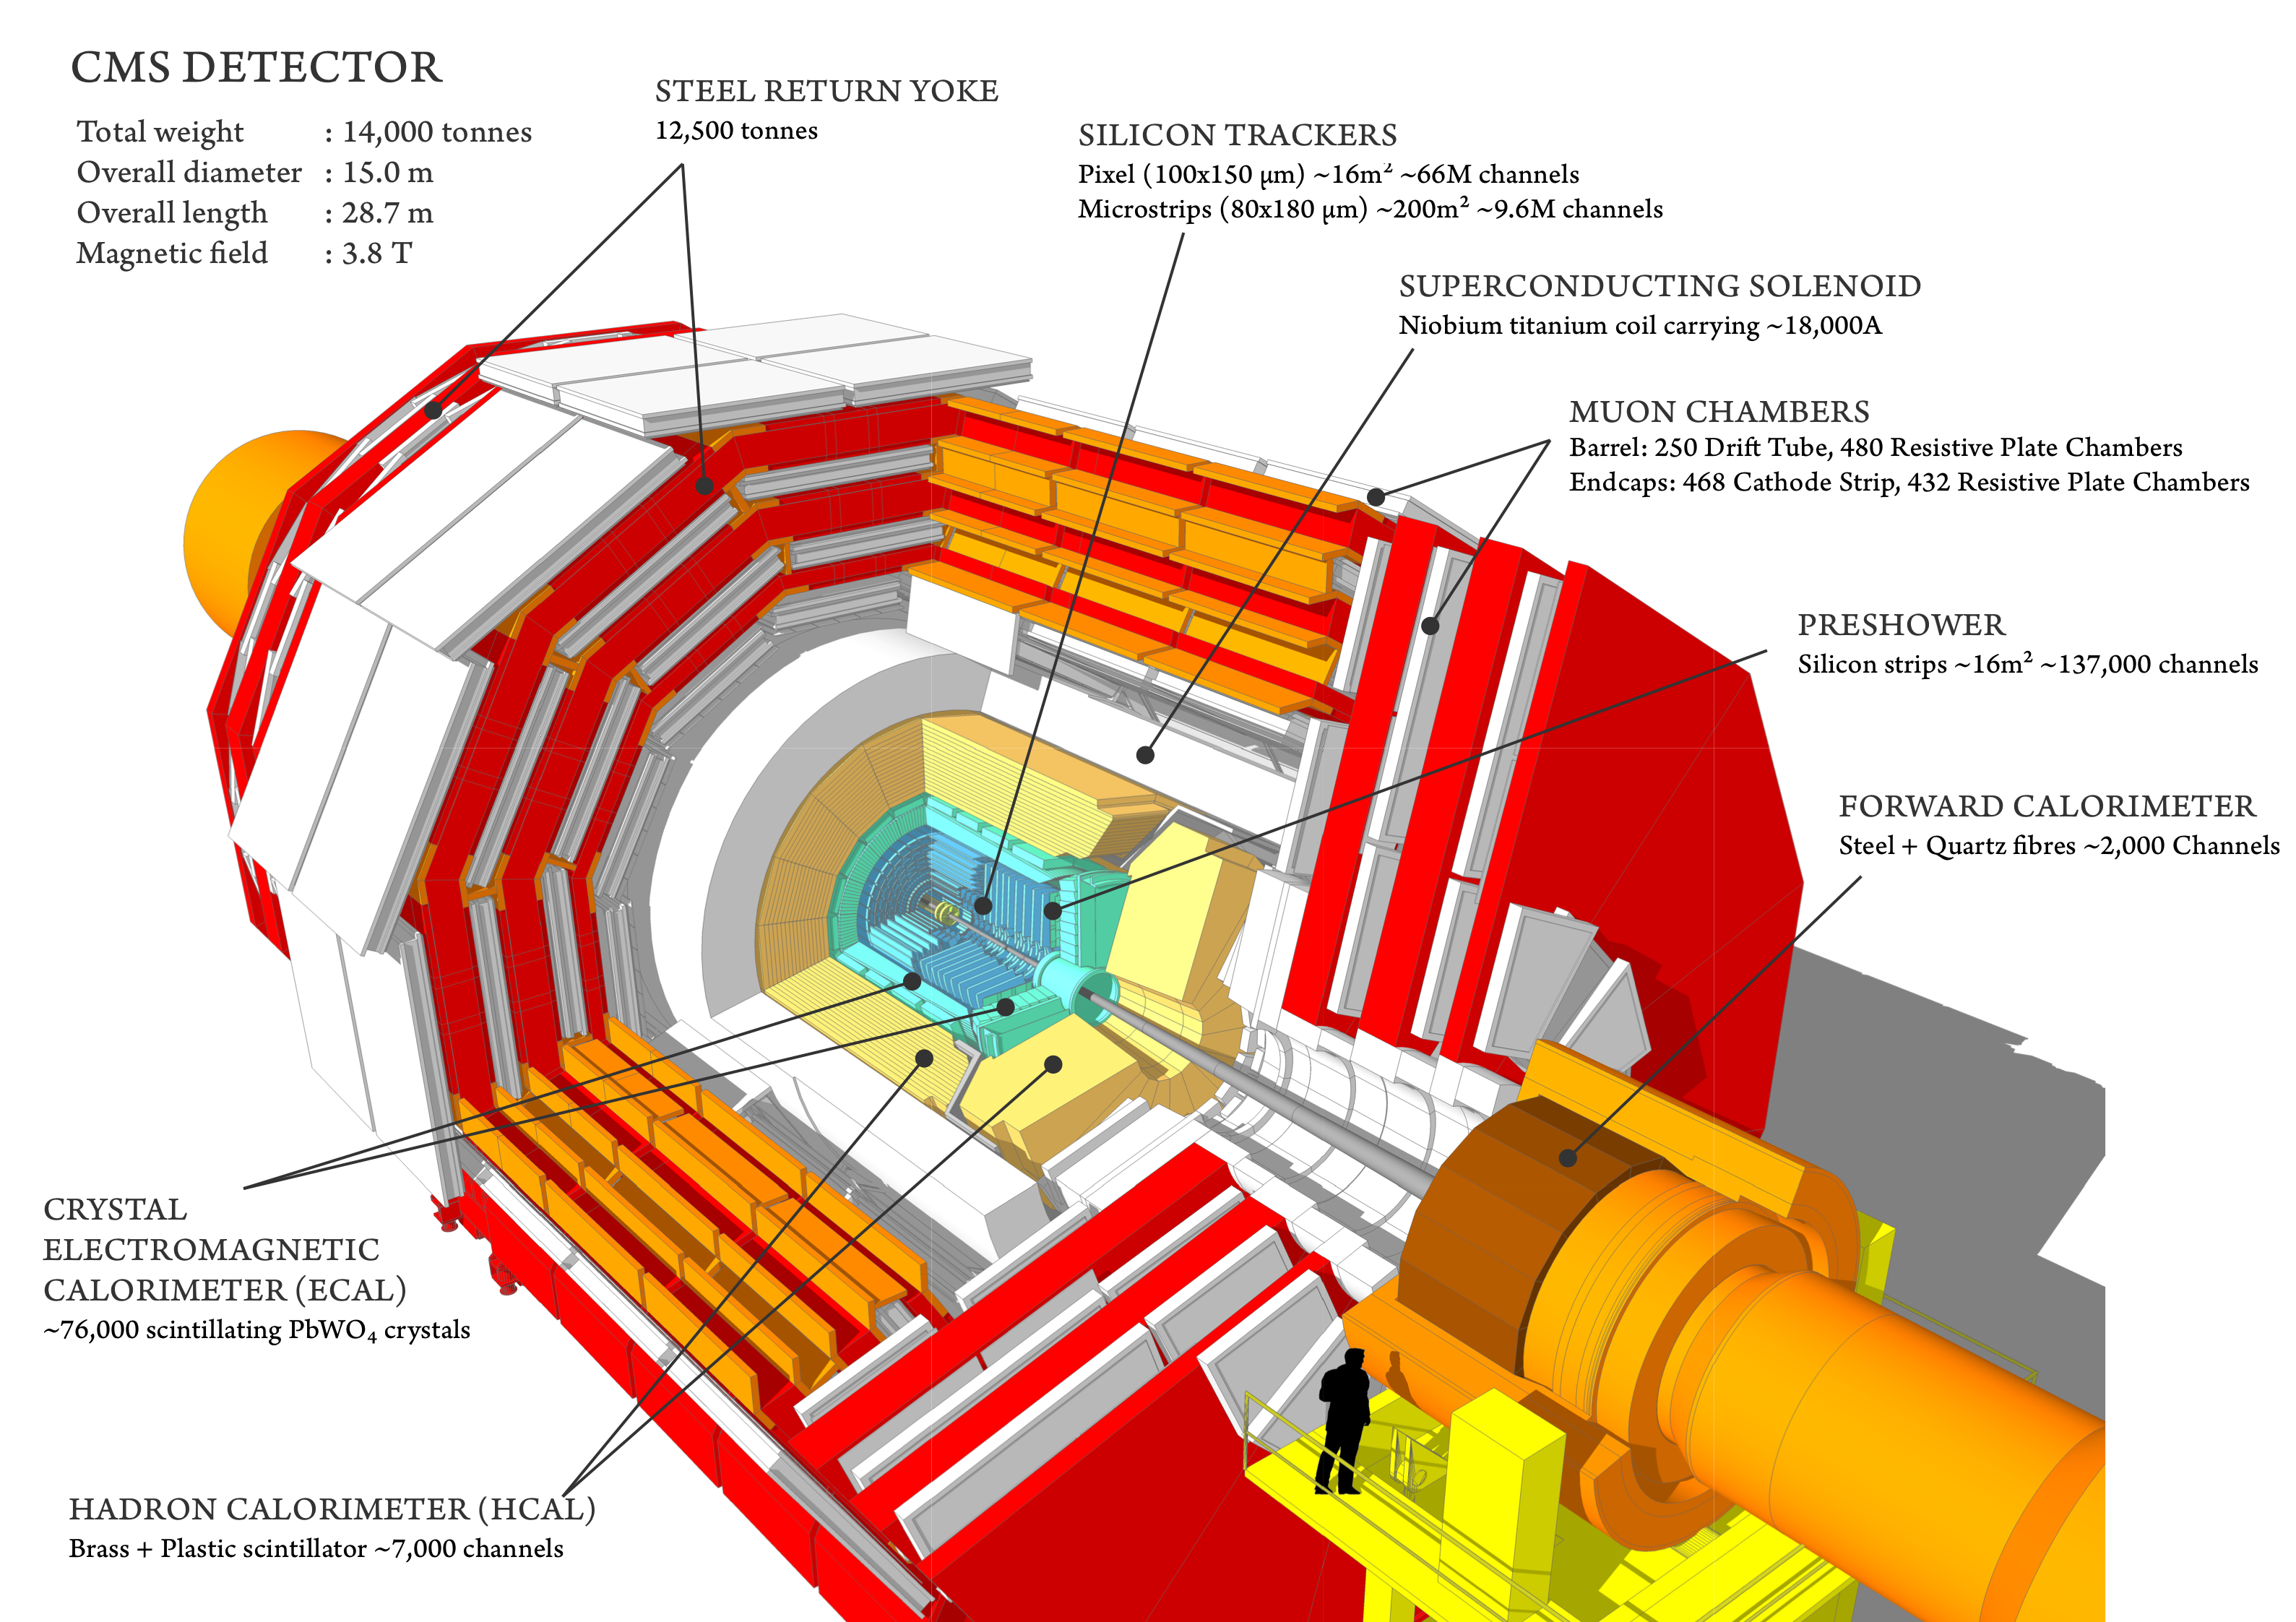
\includegraphics[height=0.49\textwidth]{introduction_figs/cms_120918_03.png}
\caption{Schematic layout of the CMS detector showing its main subsystems.}
\label{figs:CMSdet}
\end{center}
\end{figure}
The Compact Muon Solenoid (CMS) is a general purpose collider detector at the LHC. A detailed description of the CMS experiment
can be found in~\cite{Chatrchyan:2008zzk}.
As shown in Fig.~\ref{figs:CMSdet},  the apparatus has an overall length of 22~m, a diameter of 15~m, and weighs 14\,000~tonnes.
The central feature of the experiment is a superconducting solenoid
of 6~m diameter. The large magnetic field of 3.8~T provided by the solenoid is essential for achieving
the very high momentum resolution that is one of the strength's of the experiment.
Within the volume of the magnet are a silicon pixel and strip tracker, a lead tungstate crystal
electromagnetic calorimeter (ECAL), and a brass/scintillator hadron calorimeter (HCAL).
The silicon tracker measures charged particles in $|\eta|< 2.5$.
For 100\GeVc\ particles, an impact parameter resolution of $\approx 15$~$\mu$m and a \pT\
resolution of about 1.5\% are achieved.
The ECAL consists of 75\,848 lead tungstate crystals covering $|\eta|< 1.479 $ in the
barrel region (EB) and $1.479 < |\eta| < 3.0$ in two endcap regions (EE).
A two-plane lead/silicon preshower detector is located  in front of the EE.
The photon energy resolution of the ECAL at  $E_{\rm T} {\approx} 60$\GeV ranges from
 1.1\% and 2.6\% in the EB region and from and from 2.2\% to 5\% in the
endcaps.
Using the particle flow algorithm, which combines information from the inner tracker
and calorimeters, the jet energy resolution achieved in \pp\ collisions typically
is 15\% at 10\GeV, 8\% at 100\GeV, and 4\% at 1\TeV,
which compares to about 40\%, 12\%, and 5\% obtained when the calorimeters alone
are used for jet finding.
Forward calorimeters extend the rapidity coverage provided by barrel and endcap detectors.

In the steel return yoke outside the magnet, detectors are embedded for muon identification.
The muon detectors cover $|\eta|< 2.4$ using three detector technologies:
drift tubes, cathode strip chambers, and resistive plate chambers.
Matching muons to tracks in the silicon tracker allows a \pT\ resolution between
1 and 5\%, for \pT\ values up to 1\TeV.

The detector operates in identical configuration for \pp\ and \PbPb\ data taking.
The main operational difference is the configuration of the two-stage trigger system.
The first level (L1) of the trigger system employs custom hardware processors
and  uses information from the calorimeters and muon detectors to select the most
interesting events in a fixed time interval of less than 4$\mu$s.
The High Level Trigger (HLT) processor farm, based on commodity hardware,
decreases the event rate to several 100~Hz for final data storage.
For heavy-ion data taking, custom reconstruction algorithms  executed in
the HLT permit the selection of events based on photon, muon, jet and
single-track signatures, in connection with global event properties such
as charged track multiplicity or energy deposited in the calorimeters.
